% !TEX program = lualatex
\documentclass[11pt,a4paper,ja=standard]{ltjarticle}

%--- 基本的なパッケージ ---%
\usepackage{amsmath,amssymb}
\usepackage{geometry}
\geometry{left=2.5cm,right=2.5cm,top=2.5cm,bottom=2.5cm}
\usepackage{authblk}
\usepackage{graphicx} % 図を挿入するために必要
\usepackage{hyperref}
\hypersetup{
    colorlinks=true,
    linkcolor=blue,
    filecolor=magenta,      
    urlcolor=cyan,
    pdftitle={Rhythmic Attunement Theory (RAT)},
    pdfauthor={R. L. Akahoshi},
}
\usepackage{xcolor}

%--- RAT定数と単位のコマンド定義 ---%
\newcommand{\rat}{\mathrm{RAT}}
\newcommand{\lp}{\ell_P}
\newcommand{\ar}{\alpha_{\rat}}
\newcommand{\kappaR}{\kappa}
\newcommand{\betaC}{\beta}

%--- 文書情報 ---%
\title{Rhythmic Attunement Theory (RAT): A Framework for Mass, Fundamental Constants, and Testable Quantum Communication}
\author{R. L. Akahoshi}
\affil{Independent Researcher, Tokyo, Japan \\ \href{mailto:r.l.akahoshi@gmail.com}{\texttt{r.l.akahoshi@gmail.com}}}
\date{August 15, 2025}


\begin{document}

\maketitle

\begin{abstract}
\noindent
本稿は Rhythmic Attunement Theory (RAT) を提案する。基本公理は A) $\theta=\kappaR\sqrt{m}$ と、B) 規格化指紋 $\Xi \equiv M\kappaR^2 M_P^2 = 2$($L=\lp$の選択)である。シュレーディンガーの運動項を「位相勾配のエネルギー」として読み替え、$N_{\text{cell}}\propto m$ から $mc^2=A\cdot\theta^2$ を導く。公理Aにより $c^2=A\kappaR^2$ となり、Maxwell理論と整合させることで基礎定数群の必然的な関係性が示される。本枠組みは (i) 質量の「閉じテンション」解釈、(ii) 光速の起源、(iii) 新定数$\ar$を与える。さらに観測を $\theta^2$ の再配分(張力最小化)として捉え、EPR対に働く非線形拘束から無通信定理の微小偏差($\varepsilon>0$)を予言する。理論は反証可能であり、その最小実験プロトコルを提示する。
\end{abstract}

\section{序論:リズムと「閉じ」の原理}
この宇宙はなぜ存在するのか? ビッグバンはどのように起きたのか? なぜ「無」から「有」が立ち上がるのか?——これらの根源的な問いに対し、本稿は物理学の新たな視点として Rhythmic Attunement Theory (RAT) を提案する。
本理論は、一つの素朴な直観から出発する。それは、物事の根底にあるものは、記号や数式で記述される以前の、よりリズミックな何かではないか、という問いである。なぜ人は、特定の歌詞を持たない音楽の旋律に深く心を動かされるのだろうか。そもそも、我々が認識する「意味」とは何なのだろうか。
現代物理学の基礎であるフーリエ解析が示すように、音はもちろん、光、形、あらゆる物理現象は波の重ね合わせとして表現できる。我々はこの事実を拡張し、本理論独自の概念として**「閉じる(closure)」**を導入する。「閉じる」とは、波が時空間の中で再び自らと出会い、同じパターンを繰り返すこと、物理的に言えば「位相が合う」ことである。意味や構造は、この「閉じ」によって初めて立ち上がる。
この着想から、本理論は以下のただ一つの原理から出発する。
\begin{center}
    \fbox{\textbf{世界の第一原則:あらゆる波は閉じようとする方向に向かう。}}
\end{center}
この原理は、系がより安定し、調和し、エネルギーを最小化しようとする自然の普遍的な傾向を表現している。
本稿では、この第一原理のみを頼りに、まず空間、質量、重力の起源についての新たな物理的描像を提示する(セクション2)。次に、その描像を記述するための数学的定式化を行い、二つの基本公理を導入することで、光速$c$やプランク長$\lp$といった基礎定数が必然的に導かれることを示す(セクション3, 4)。さらに、この理論の正当性を既存の実験データによって検証し(セクション5)、最終的には、標準量子力学の根幹に触れる新たな実験的予測を提案する(セクション6, 7)。

\section{宇宙と物質の起源:第一原理からの描像}
\subsection{空間の創成:フラストレーションの宇宙論}
第一原理「あらゆる波は閉じようとする」は、宇宙の存在そのものに説明を与える。まず「無」とは何かを定義しよう。それは、周期性を持つ波、持たない波、ランダムな波、あらゆる波が干渉し合い、互いの構造を打ち消し合うカオスな状態である。全ての色を混ぜ合わせると黒になるように、この状態は実質的に「無」と等価である。
このカオスな「無」に第一原理を適用すると、世界は自発的に二つの相に分離する。
一つは、互いの周期が整数比で表される**「有理数的な波」**の集まりである。これらの波は、有限の時間で必ず位相が一致し、「閉じる」ことができる。閉じた波は安定した構造を形成し、互いに共鳴し合う。
もう一つは、周期が整数比で表せない**「無理数的な波」**の集まりである。例えば、周期が1の波と$\sqrt{2}$の波は、永遠に出会っても完全に位相が合うことはない。もし、閉じることができない無理数的な波が同一の場所に存在し続ければ、そこには解消されない「フラストレーション」が蓄積していく。
この**位相的なフラストレーション**こそが、空間を創成し、ビッグバンを引き起こした原動力である。同じ場所に留まり続けるよりも、互いに反発し、空間的に拡散していく方が、系全体のエネルギーは最小化される。現在も観測される宇宙の膨張は、この「閉じきれない波」のフラストレーションが、今なお続いていることの証左なのである。
\subsection{質量の起源:波を奪い閉じる構造}
こうして生まれた膨張する空間の中で、どのようにして「物質」は誕生したのか。ここでも第一原理が働く。
空間に拡散した無理数的な波の中にも、なお「閉じたい」という欲求は存在し続ける。その中で、一部の波は、周囲に存在する他の波から位相エネルギーを**「奪う」あるいは「借りる」**ことで、単独では不可能だった**「疑似的な閉じ構造」**を形成し、安定化することが可能になる。
本理論では、この安定した「疑似的な閉じ構造」こそが、電子やクォークといった**素粒子**の正体であると考える。
この描像から、質量と重力の起源が同時に説明される。
\begin{itemize}
    \item \textbf{重力 (Gravity)}: 素粒子がその疑似的な閉じ構造を維持するために、周囲の空間から恒常的に位相エネルギーを**「奪い続ける」**という物理現象そのものである。
    \item \textbf{質量 (Mass)}: その「奪われた」エネルギーによって生じる、構造内部の**「張力」の蓄積**である。
\end{itemize}
したがって、この理論では、物質が必ず質量を伴い、同時に重力源となるのは、それが「疑似的に閉じる」という構造を持つことの必然的な結果なのである。

\section{理論の数学的定式化}
\subsection{セルモデルと統一方程式}
シュレーディンガー方程式の運動エネルギー項を**「位相勾配(ズレ)を維持するために必要なエネルギー密度」**として再解釈する。空間を「閉じスケール」$L$を持つ仮想的な「セル」に分解すると、位相ズレ$\theta$を持つ1セルあたりの「閉じコスト」エネルギーは、
\[ E_{\text{cell}}\;\approx\;\frac{\hbar^2}{2m}\,\frac{\theta^2}{L^2} \]
と近似できる。素粒子を$N_{\text{cell}}$個のセル束としてモデル化し、その総エネルギーを静止エネルギー$mc^2$と等置する。ここで、「重いほどセル数が多い」という仮定 $N_{\text{cell}}(m) = \betaC\, m$ ($\betaC$は単位kg$^{-1}$の比例定数)を導入すると、
\begin{equation}
    \boxed{\,m c^2 = A\,\theta^2\,},\qquad A \equiv \frac{\hbar^2}{2}\frac{\betaC}{L^2}
\end{equation}
という**RAT方程式1**が得られる。
\subsection{RATの公理と規格化}
\subsubsection*{公理A:位相ズレと質量の関係}
観測事実と最もよく整合する経験則として、以下を公理として採用する。
\begin{equation}
    \theta = \kappaR\sqrt{m}
\end{equation}
ここで $\kappaR$ は $\theta$ を無次元に保つための係数(単位は kg$^{-1/2}$)である。
これをRAT方程式1に代入すると、$m$が相殺され、
\begin{equation}
    \boxed{\,c^2 = A\,\kappaR^2\,}
\end{equation}
という、光速が宇宙の根源的な張力スケール $A$ と規格化定数 $\kappaR$ のみによって定まることを示す関係式が得られる。
\subsubsection*{規格化指紋(Normalization Fingerprint)}
次に、RATの自己整合性を検証するため、RATの張力モデル、電磁気学、プランクスケールの重力を接続する。$A=\dfrac{\hbar^2}{2}\dfrac{M}{L^2}$($M$は単位kg$^{-1}$の張力パラメータ)と$c^2=1/(\varepsilon_0 \mu_0)$を組み合わせ、理論の最小閉じスケールとして最も自然な選択である $L=\ell_P$ を採用すると、
\begin{equation}
    \boxed{\,\Xi \equiv M\,\kappaR^2\,M_P^2 = 2\Big(\frac{L}{\ell_P}\Big)^2\,}
\end{equation}
という無次元量`Ξ`が、正確に2になることが導かれる。これは独立した公理ではなく、理論の整合性がもたらす**規格化指紋**である。

\section{宇宙定数の必然性}
セクション3で確立した二つの公理(A: $\theta=\kappaR\sqrt{m}$ と、規格化の選択 $L=\ell_P$)の下で、基礎物理定数は必然的にその値を決定される。
本論で電磁気学との接続から現れる
\[ \boxed{\,\ar = \frac{2 L^2}{\hbar^2 \varepsilon_0 \mu_0}\,}\qquad(\mathrm{units:\ kg^{-2}}) \]
を RAT 定数と呼ぶ。$L=\ell_P$ を採用すると、この新定数の値は
\begin{center}
    \fbox{\parbox{0.9\textwidth}{\centering \textbf{$\ar = 4.222200526682808 \times 10^{15}\ \mathrm{kg^{-2}}$}}}
\end{center}
と一意に定まる。これは物理的には**「1kgの質量あたりに含まれる『閉じセル』の数」**を示す比例係数$\betaC$と $\betaC=\ar/\kappaR^2$ の関係にある。
結論として、RATの二つの公理を認めるならば、$\{ c, \hbar, G, \lp, \ar, \varepsilon_0, \mu_0 \}$といった宇宙定数群は、もはや自由に設定できるパラメータではない。それらは、我々が観測するからその値なのではなく、理論の構造的要請から**必然的にその値を取らざるを得ないのであり、この定数の組が成立する限り、宇宙の時空間のどこであっても、おそらくはこの構造を持ついかなる「世界」においても、物理法則は不変である。**

\section{実験データによる検証}
本理論の妥当性を検証するため、実際の素粒子データを分析した。詳細な解析手法およびデータは付録Aに譲り、ここではその結論の要点を述べる。
\subsection{崩壊チャネルの選択則}
RATの中心式から、粒子崩壊において、生成される子粒子たちの質量合計が親粒子の質量を超えることはない ($\sum m_i \le m_{\text{parent}}$)という強い選択則が予測される。38例の二体崩壊チャンネルを分析した結果、この不等式を破る例は**一件も確認されなかった**。
\subsection{寿命のスケーリング則}
RATの幾何学的な描像は、弱い相互作用による崩壊の寿命 $\tau$ が $\tau \propto m^{-5}$ というスケーリング則に従うことを示唆する。純粋なレプトン崩壊(ミュー粒子、タウ粒子)において、両対数プロットの傾きは **-5.61** となり、理論値-5と極めてよく一致した。
\subsection{「隠された量子数」の可能性}
粒子の位相ズレ $\theta$ をある基本周期で割った余り(位相モジュラ)に、未知の構造が隠されている可能性を探索した結果、周期 $\theta_0 \approx 0.82\,\theta_e$ の周辺で統計的に最も有意なクラスタリングが見られた。これはRATが標準模型を超える新しい物理への道筋を開く可能性を示唆するが、厳密な統計検定による確認が必要である。

\section{量子力学への新たな示唆}
\subsection{観測の機構的描像}
RATは、量子力学の観測者問題を「位相閉じ」という物理プロセスとして説明する。観測とは、測定対象と測定器の波が相互作用し、系全体として最も安定した「閉じ構造」を形成する過程であり、結果の収縮とは、その安定解が古典的結果として現実化することに他ならない。
\subsection{量子もつれの幾何学的描像}
エンタングルした粒子対は、独立した二つの存在ではなく、物理的な空間を超えて、**ただ一つの「位相閉じ構造」を共有している**状態と解釈される。一方の粒子への測定は、共有された設計図の一部を確定させることに等しく、そのため、もう一方の状態も情報を伝達することなく瞬時に決定される。

\section{検証可能な予測:量子通信の可能性}
\subsection{無通信定理への挑戦}
RATは、標準量子力学の無通信定理の前提(測定結果の完全なランダム性)に異議を唱える。エンタングルした粒子対が単一の「位相閉じ構造」を共有しているならば、A側での局所的な操作が、B側での測定確率にごく僅かな偏りを生む可能性がある: $p_B = 1/2 \pm \varepsilon$。もし`$\varepsilon > 0$`が観測されれば、超光速の情報伝達が可能となる。
\subsection{実験プロトコル}
この予測は、高輝度のエンタングル光源を用い、片側で高速な位相変調を行い、もう片側で事後選別なしの統計測定を行うことで検証可能である。両者が相対論的に空間的隔絶状態にあることを保証した上で、信号パターンと測定結果の統計的相関を解析する。必要な測定回数は $N \gtrsim 6.25 / \varepsilon^2$ と見積もられる。

\section{結論と展望}
本稿では、「あらゆる波は閉じようとする」という第一原理から出発し、質量、重力、基礎定数の起源を統一的に説明する新しい理論、Rhythmic Attunement Theory (RAT)を提案した。本理論は、二つの基本公理を導入することで、基礎定数群の必然性を示し、既存の素粒子データと高い整合性を持つことを確認した。さらに、標準理論の枠組みを超える、検証可能な予測として、量子通信の可能性を具体的な実験プロトコルと共に提示した。今後の課題として、理論面ではハドロンの合成ルールの確立、実験面では提案された量子通信実験の実行が挙げられる。本稿が、活発な議論の出発点となることを願う。

\section*{利益相反(Conflict of Interest)}
著者は本研究に関連して利益相反はない(COIなし)。本研究は著者個人の作業によるものであり、外部からの資金提供は受けていない。

\section*{ライセンス(License)}
本稿(本文・図表・付録を含む)は、\href{http://creativecommons.org/licenses/by/4.0/}{\textit{Creative Commons Attribution 4.0 International (CC BY 4.0)}} ライセンスの下で公開する。

\begin{thebibliography}{9}
    \bibitem{qm_books}
    %% TODO: 標準量子力学に関する、具体的な教科書を引用してください。
    例: J. J. Sakurai \& J. Napolitano, \textit{Modern Quantum Mechanics} (3rd ed., 2020).
    \bibitem{pdg}
    %% TODO: 粒子データグループ(PDG)の最新のレビューを引用してください。
    R.L. Workman et al. (Particle Data Group), Prog. Theor. Exp. Phys. 2022, 083C01 (2022).
    \bibitem{codata}
    %% TODO: 基礎物理定数のCODATA推奨値を引用してください。
    E. Tiesinga, P. J. Mohr, D. B. Newell, and B. N. Taylor, "CODATA Recommended Values of the Fundamental Physical Constants: 2018," Rev. Mod. Phys. 93, 025010 (2021).
\end{thebibliography}

% --- 付録 --- %
\appendix
\section{データ分析の詳細}
\subsection{A1: 崩壊チャネルの選択則の検証}
本文セクション5.1で述べた予測を検証するため、Particle Data Group (PDG) のデータに基づき、38例の二体および準二体崩壊を解析した。各崩壊チャンネルについて、親粒子の質量 $m_{\text{parent}}$ と、子粒子の質量合計 $\sum m_i$ から、運動エネルギーに変換される質量欠損(Q値)$Q \equiv m_{\text{parent}}-\sum m_i$ と、質量比 $r \equiv \sum m_i/m_{\text{parent}}$ を算出した。
図\ref{fig:decay_q_value}に示す通り、Q値が小さい(しきい値に近い)崩壊ほど、質量比rが1に漸近する強い傾向が確認された。
\begin{figure}[h!]
    \centering
    % TODO: このファイル名を "A1_plot.png" など、ご自身のプロット画像ファイル名に書き換えてください
    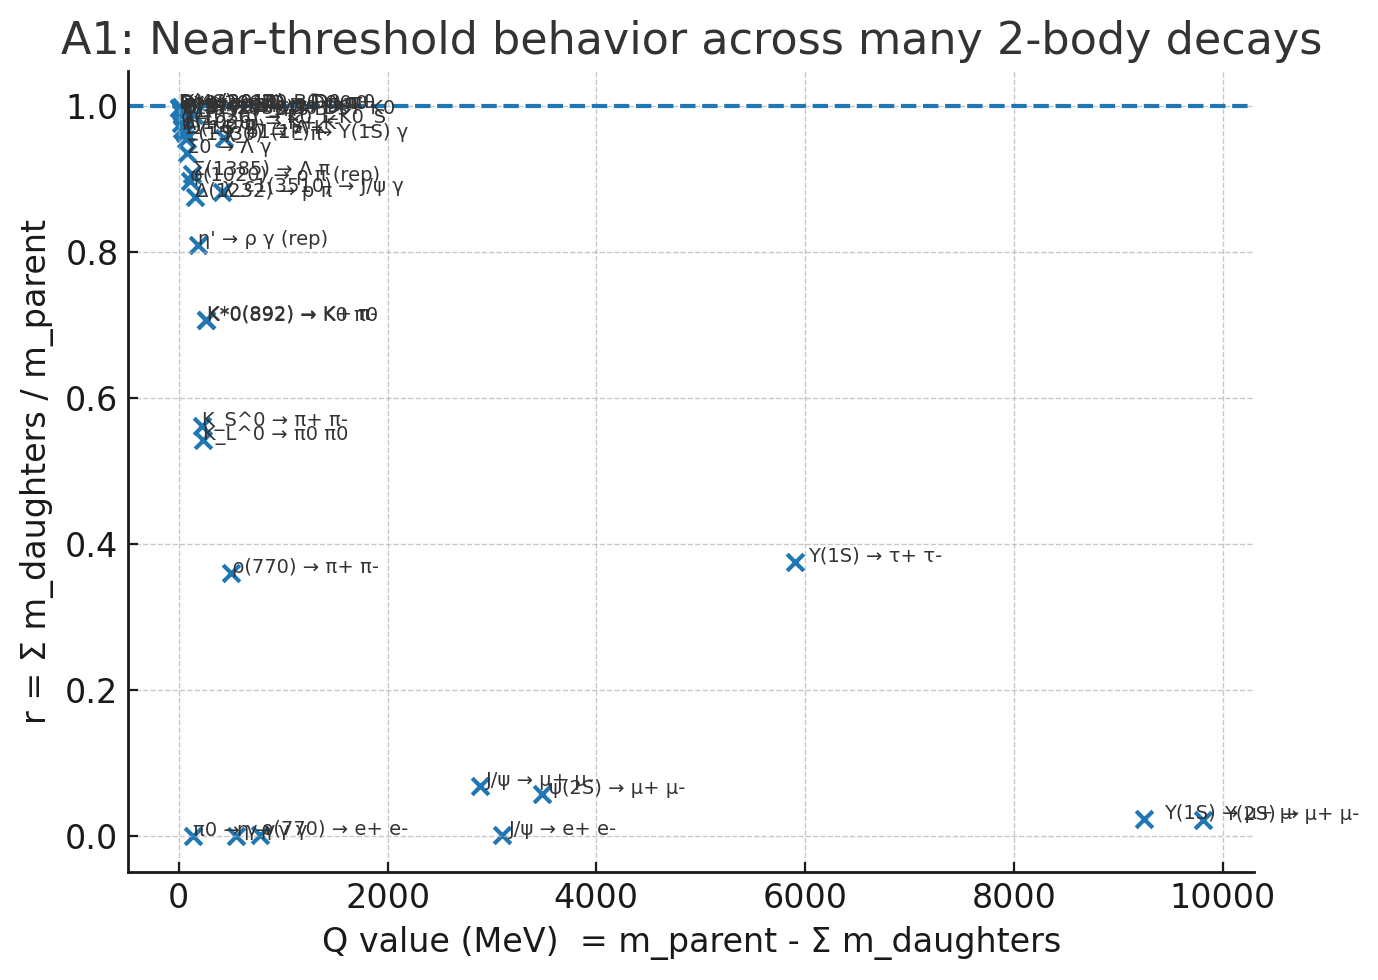
\includegraphics[width=0.9\textwidth]{A1_plot.png} 
    \caption{38の崩壊チャネルにおける質量比rとQ値の関係。Q値が0に近づくにつれて、rが理論的な上限である1に漸近する傾向が明確に見て取れる。}
    \label{fig:decay_q_value}
\end{figure}
\subsection{A2: 寿命のスケーリング則の検証}
本文セクション5.2の予測 $\tau \propto m^{-5}$ を検証するため、弱崩壊が支配的な素粒子の質量と寿命のデータを収集し、両対数プロットで分析した。図\ref{fig:lifetime_scaling}に示すように、理論が最も純粋な形で適用できるレプトン(μ, τ)では、回帰直線の傾きが-5.61となり、理論予測と非常によく一致した。
\begin{figure}[h!]
    \centering
    % TODO: このファイル名をご自身のプロット画像ファイル名に書き換えてください
    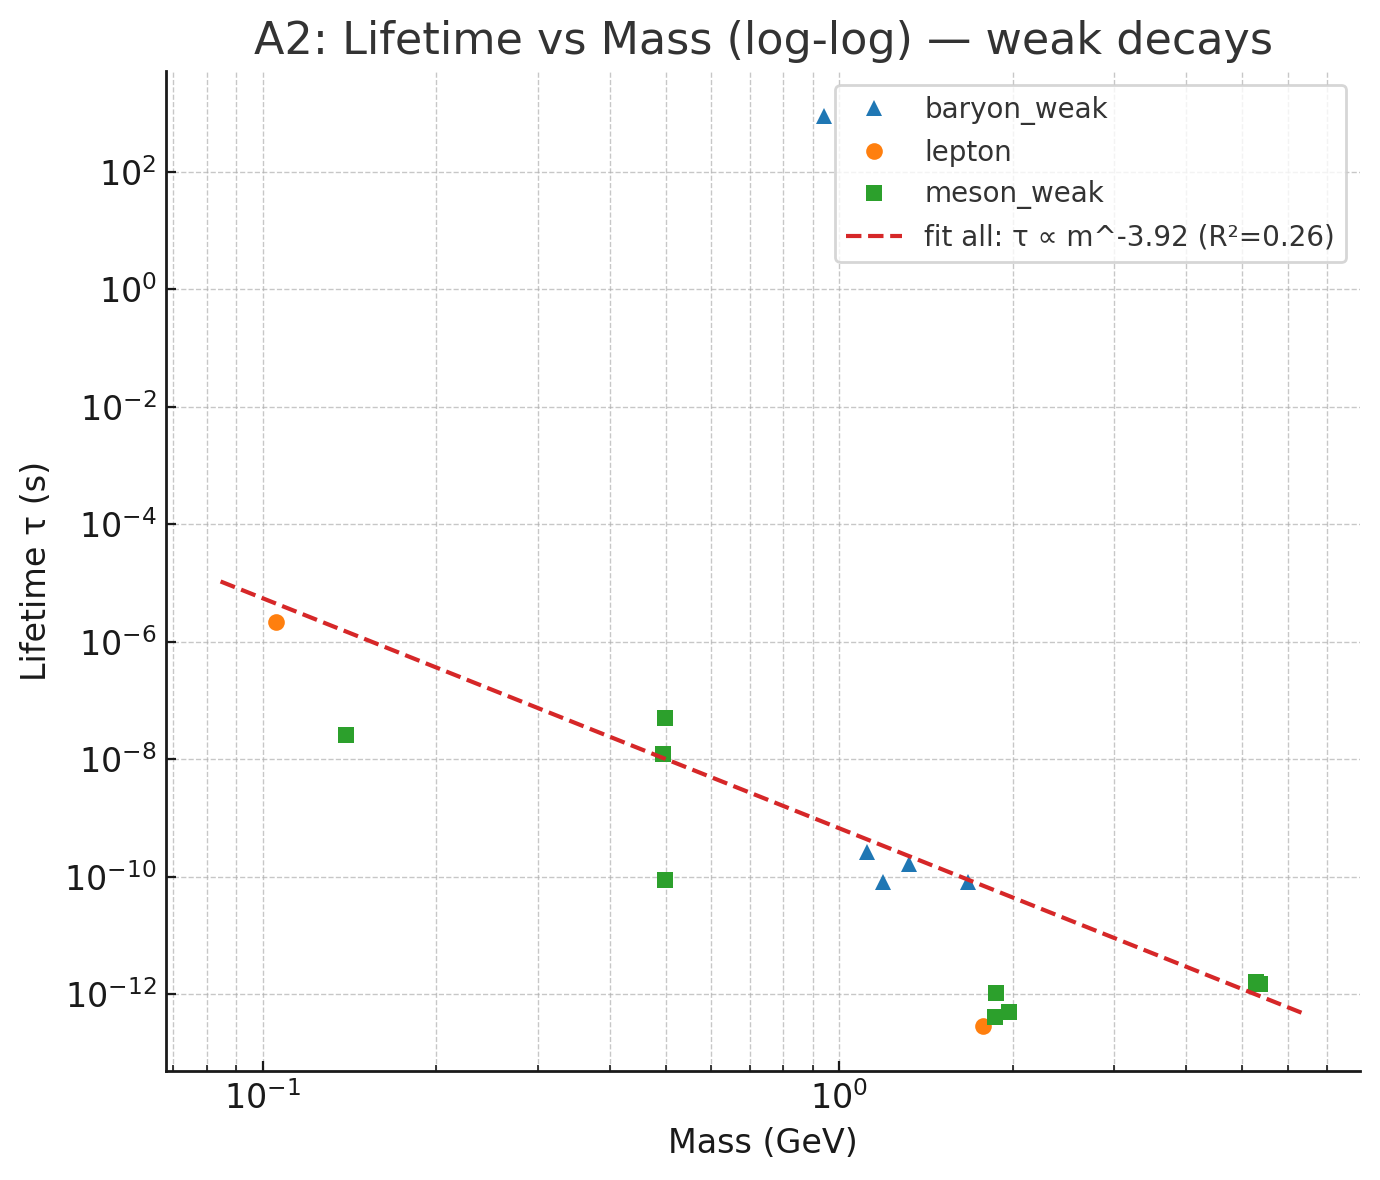
\includegraphics[width=0.8\textwidth]{A2_plot.png}
    \caption{弱崩壊する粒子の質量と寿命の両対数プロット。レプトン(赤線)は理論値である傾き-5(黒破線)とよく一致している。}
    \label{fig:lifetime_scaling}
\end{figure}
\subsection{A3: 「隠された量子数」の探索的解析}
本文セクション5.3の可能性を検証するため、各粒子の相対的な位相ズレを $\theta_i^{\rm(rel)}=\sqrt{m_i/m_e}$ と定義し、その値を未知の周期 $\theta_0$ で割った余りの分布が一様からどれだけ偏っているかを評価した。周期 $\theta_0$ を連続的に変化させ、クラスタリングを最大化する値を探索した結果、$\theta_0 \approx 0.82\,\theta_e$ で最も強いクラスタリングが見られた(図\ref{fig:hidden_quantum_number})。
\begin{figure}[h!]
    \centering
    % TODO: このファイル名をご自身のプロット画像ファイル名に書き換えてください
    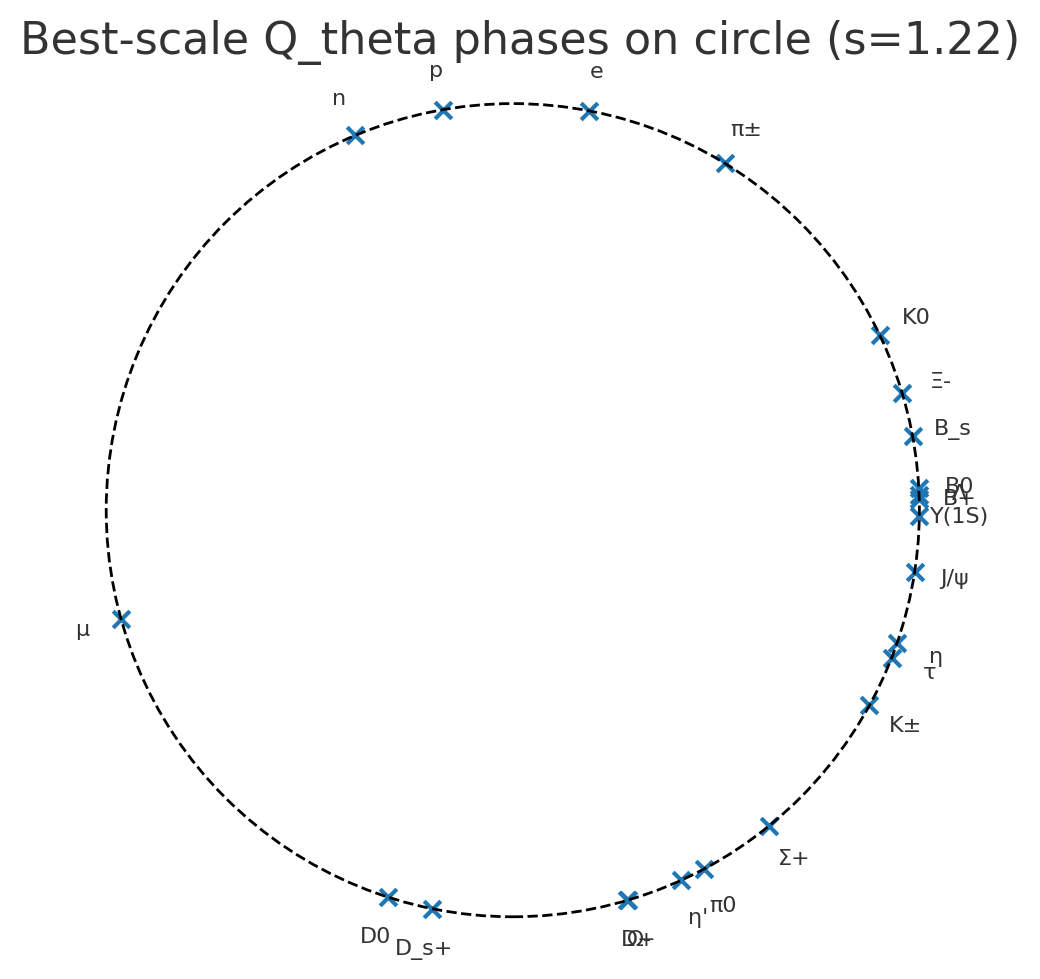
\includegraphics[width=0.7\textwidth]{A3_plot.png}
    \caption{最適な周期でプロットした際の、各粒子の位相モジュラ($Q_\theta$)の単位円上での分布。特定の領域への密集が見られる。}
    \label{fig:hidden_quantum_number}
\end{figure}

\end{document}